\documentclass[../main/main.tex]{subfiles}

\begin{document}
\section{Diffusion law}
\subsection{Non-equilibrium thermodynamics}
\newdate{date}{15}{03}{2023}

\marginpar{ \textbf{Lecture 4.} \\  \displaydate{date}. \\ Compiled:  \today.}

\begin{wrapfigure}{l}{0.5\textwidth}
    \centering
    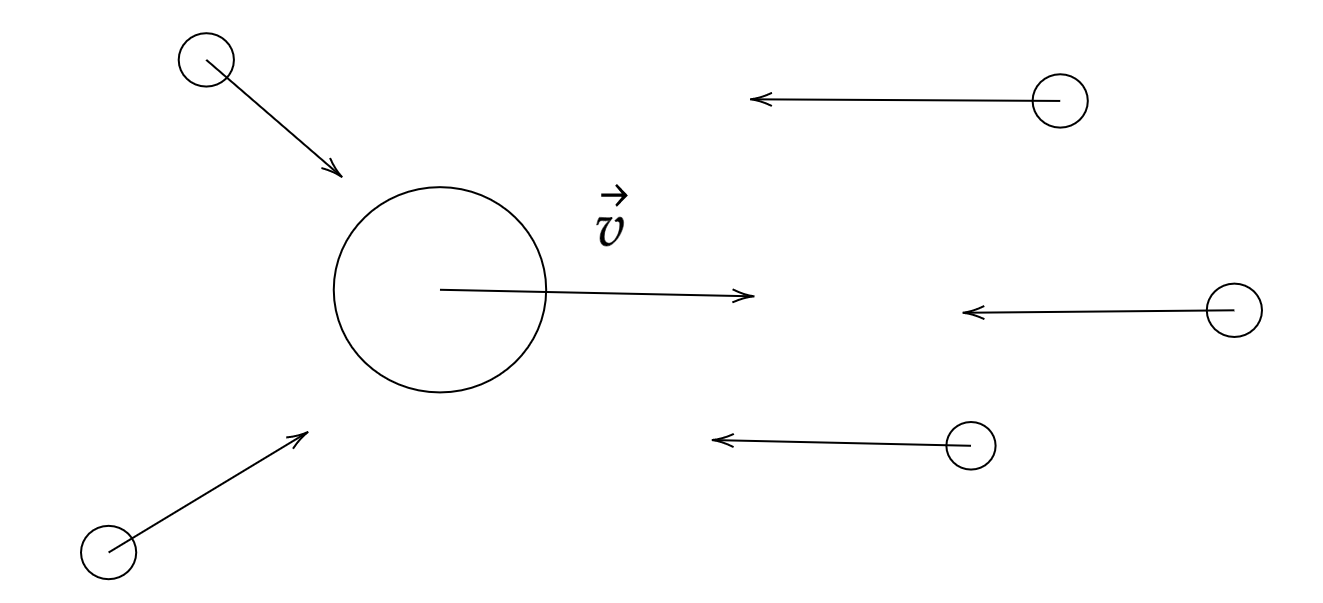
\includegraphics[width=0.5\textwidth]{../frontespizio/tikz/5_lesson/friction.png}
    \caption{\label{fig:friction} Friction caused by water molecules.}
\end{wrapfigure}

We will deal now with the dffusion law, from a Lagrangian perspective. \\
In doing this, we now have to take care of \emph{viscosity} and \emph{friction}: since bodies move in water, they are slowed down by collisions. The motion of our particle remains a stochastic one to which also water molecules collaborate, both in the diffusion process and in a friction process.
We will use the Navier-Stokes quation, just as a reference equation, without deriving it. 

In general in thermodynamics, the gradient of an \emph{intensive} variabile is related to the so called \emph{generalized thermodynamic force}, whihc effect is to to generate a \textbf{flux} of an \emph{extensive} varibale, which satisfies a balance equation (equation [\ref{eq:balance_equation}]). So, the gradient of an intensive variable is related to the flux of an extensive variable, through a \emph{consitutive} or \emph{material relation} and appositely introduced transport coefficients, thermodynamics quantities involving time. We have to think of this as a Taylor expansion truncated at the first term, in order to consider the so called \emph{linear non-equilibrium thermodynamics} approximation, when we are able ti work close to the equlibrium point.
Just to give some examples, we can think of the \emph{temperature gradient} which is related to the \textbf{heat flux} which introduces also the coefficient of thermal conductivity, or the \emph{electric potential gradient} to which it is associated the \textbf{charge flux} which introduces the electric conductivity coefficient. An intensive quantity that plays a key role in this subject is for sure the \emph{concentration of particle}, which gradient is related to the \textbf{number flux} and the already seen introduction of a transport coefficient, the diffusion coefficient.

\begin{table}[h!]
    \centering
    \caption{Generalized theromodynamic forces}
    \label{generalized theromodynamic forces}
    % \resizebox{\textwidth}{!}{%
    \begin{tabular}{l|l|l}
    Intensive gradient & Flux of extensive variable & Physical laws \\ \hline
    Temperature $T$ & Heat $Q$ & Fourier's law \\
    Electric potential $V$ & Electric $\Phi$ & Ohm's law \\
    Concentration $c$ & Number of particles $j$ & Fich's diffusion law
    \end{tabular}%
    % }
\end{table}
Another important example is the \emph{Shear velocity tensor} or \emph{rate of shear strain}, which is the rate of change of the deformation - \emph{shear} is the deformation of a solid with respect to some equilibrium position - that is a varying parameter when dealing with liquids. The associated flux is the \textbf{momentum flux}, called also the \textbf{stress tensor} - a tensor is needed since now momentum is a vector quantity - snd the transport coefficient associated is the so called \textbf{viscosity coefficient}.

\subsection{Coutte simple experiment}

\begin{figure}[h!]
    \centering
    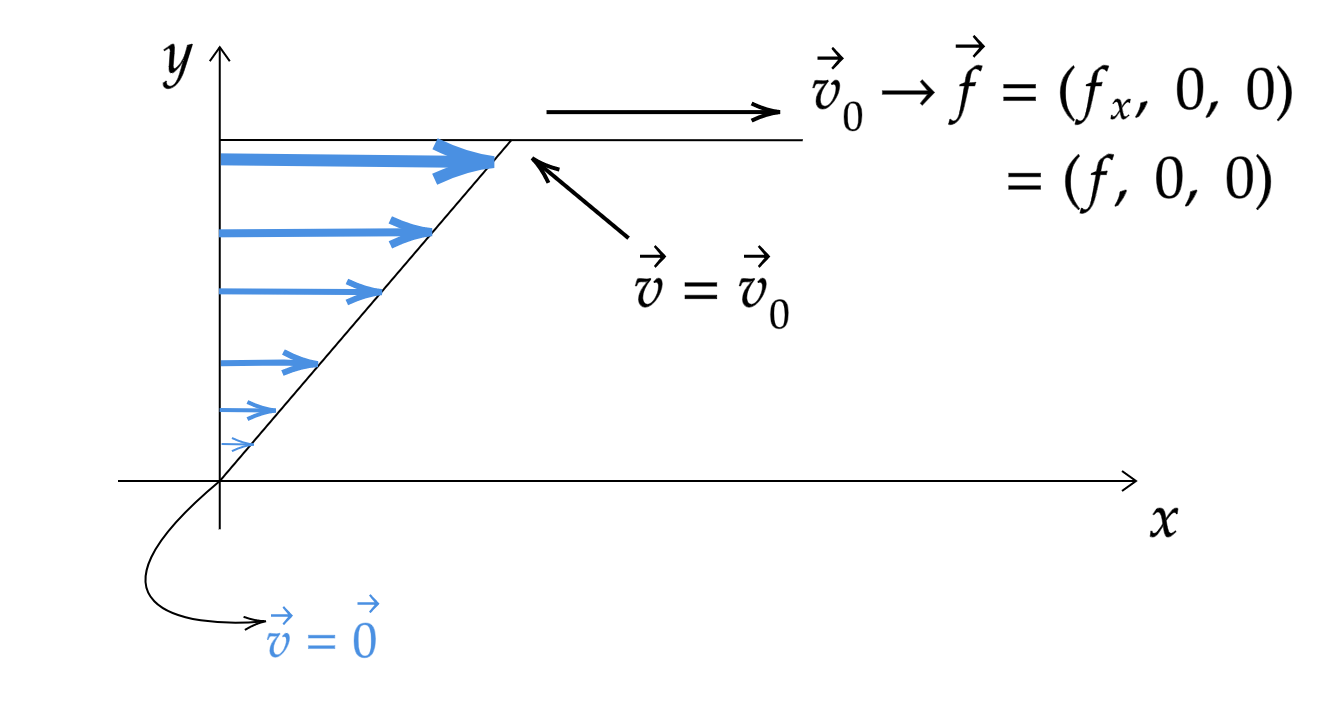
\includegraphics[width=0.7\textwidth]{../frontespizio/tikz/5_lesson/couette.png}
    \caption{Simple Coutte flow}
\end{figure}
In this experiment we have a fluid constrained between two boundary planes: the one at the top, at a height $d$ moving to the right, and the one at the bottom at rest. Because of viscosity, the moving of the upper plane will cause the movement of the fluid, inducing a linear velocity field $\vec{v}(\vec{r})$ in the fluid itself. The fluid moves at $\vec{v}=\vec{v}_0$ at $y=d$ and it is at rest at $y=0$, considering \emph{no-slip boundary conditions}.
Due to the presence of an external drag force $\vec{f}=(f, 0, 0)$ along the $x$ axis, the out of equilibrium extensive variable is the vector field $\vec{v}(\vec{r})=(v_x(y), 0, 0)$. The associated generalized force is the shear velocity tensor:
\begin{equation*}
    (\vec{\nabla}\vec{v})_{xy} + (\vec{\nabla}\vec{v})_{yx} = \frac{\partial v_x(y)}{\partial y}+\cancel{\frac{\partial v_y(x)}{\partial x}} = \frac{\partial v_x(y)}{\partial y}
\end{equation*} 
which represents the generalized thermodynamic force. If we now consider the flux of $p_x$ along the $y$ direction, so passing through a surface perpendicular to the $y$ axis, we obtain the \emph{stress tensor} 
\begin{equation}
    \tau_{xy} =\underbrace{\frac{1}{A_y}\:\frac{\partial p_x}{\partial t}}_{\text{flux term}} = \frac{1}{A}\: f_x = \underbrace{\frac{f}{A}}_{\text{pressure term}} 
    \label{eq_constitutive_equation}
\end{equation} 
The constitutive relation introduces the \textbf{shear viscosity coefficient} $\eta$, given by $\tau_{xy}=\eta \frac{\partial v_x(y)}{\partial y}$ which dimension is $[\eta]=[P]\mathbb{T}=\frac{\mathbb{M}}{\mathbb{LT}}$ and for water it is $\eta_{H_2 O}=10^{-3}Pa\cdot s$.
It is worth underlying that we will only consider \emph{newtonian fluids}, so where $\eta$ is independent of thermodynamic forces, so $\eta$ is independent of the rate of shear strain $\frac{\partial v_y}{\partial y}$. This viscosity coefficient is in fact a \emph{shear} viscous coefficient, since in this experiment we are imposing the boundary of stressing the fluid through its shear component. We could have also imposed a stress perpendicular to the surface of the fluid, but in this case we would have considered the \textbf{bulk} effect, so a friction effect with respect to a deformation perpendicular to the $y$ axis.
But, for incompressible fluids, for which we can state the equation 
\begin{equation*}
    \vec{\nabla}\cdot\vec{v}=0
\end{equation*}
bulk viscous effect does not play any role, so they are negligible in the Navier-Stokes equations. 
We put all of these constrains mainly because water is both a newtonian and an incompressible fluid!

\section{Stokes' law}
\begin{wrapfigure}{l}{0.5\textwidth}
    \centering
    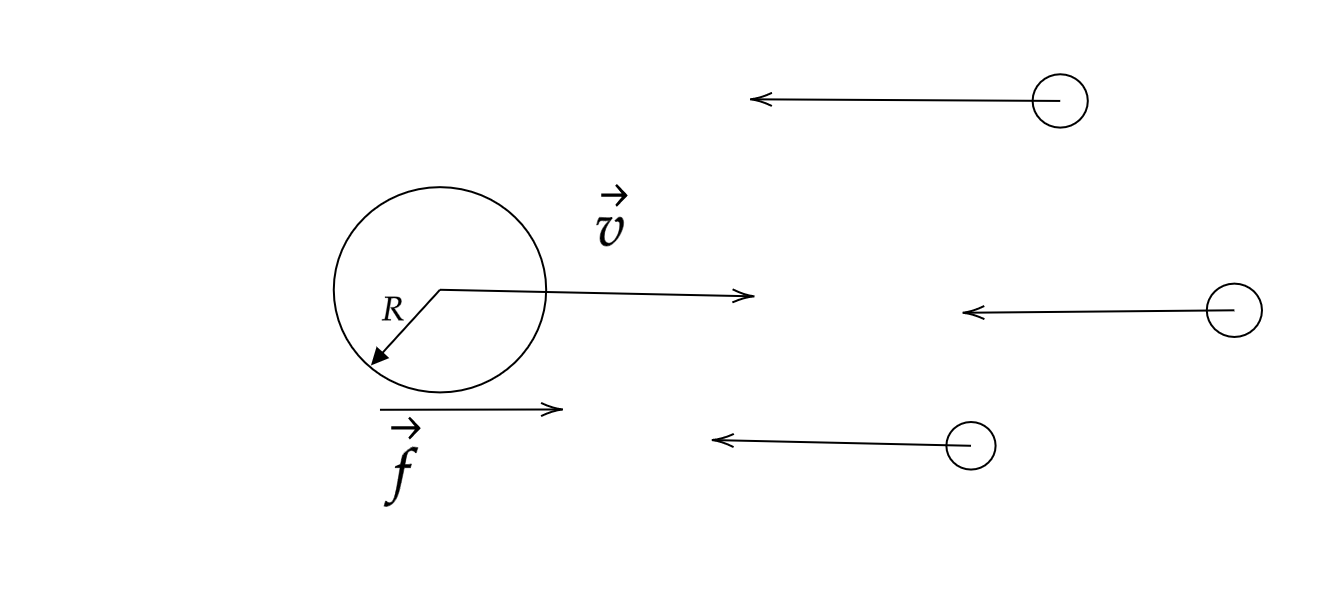
\includegraphics[width=0.6\textwidth]{../frontespizio/tikz/5_lesson/Stokes_law.png}
    \caption{\label{fig:stokes} Stokes' law.}
\end{wrapfigure}


\end{document}